\documentclass[border=12pt]{standalone}
\usepackage[T1]{fontenc}
\usepackage{helvet}
\renewcommand{\familydefault}{\sfdefault}
\usepackage{amsmath}
\usepackage{tikz}
\usetikzlibrary{positioning,arrows.meta,calc,fit,backgrounds,shapes.geometric,shapes.misc}

% palette
\definecolor{spinefill}{RGB}{232,234,238}
\definecolor{spinedraw}{RGB}{110,118,130}
\definecolor{liverfill}{RGB}{246,247,249}
\definecolor{liverdraw}{RGB}{168,175,184}
\definecolor{teald}{RGB}{13,110,122}
\definecolor{tealfill}{RGB}{223,239,240}
\definecolor{amber}{RGB}{193,118,18}
\definecolor{amberfill}{RGB}{250,240,222}
\definecolor{inkc}{RGB}{33,38,46}
\definecolor{salmon}{RGB}{193,110,95}
\definecolor{salmonfill}{RGB}{244,225,220}

% badges
\newcommand{\bnew}{\colorbox{teald}{\textcolor{white}{\scriptsize\bfseries NEW}}\hspace{2pt}}
\newcommand{\bchg}{\colorbox{amber}{\textcolor{white}{\scriptsize\bfseries CHANGED}}\hspace{2pt}}

\begin{document}
\begin{tikzpicture}[
  card/.style={rounded corners=4pt, draw, line width=0.8pt, inner sep=0pt},
  hd/.style={font=\bfseries, text=white, align=center},
  bul/.style={align=left, font=\small, text=inkc, inner sep=0pt},
]
\def\lw{7.0}   % panel width
\def\lh{9.2}   % panel height

% ===== title =====
\node[align=center, font=\large\bfseries, text=inkc] at (0,5.15)
  {Why the pipeline diverged: a harder imaging regime};

% ===== LEFT: liver =====
\begin{scope}[shift={(-4.05,0)}]
  \node[card, draw=liverdraw, fill=liverfill, minimum width=\lw cm, minimum height=\lh cm] (Lc) at (0,0){};
  \node[card, fill=liverdraw, minimum width=\lw cm, minimum height=0.95cm, anchor=north] at (Lc.north){};
  \node[hd] at ($(Lc.north)+(0,-0.47)$) {LIVER EM\\[-1pt]\footnotesize\mdseries vascular \& cellular structures};
  % schematic: compact, well-separated blobs
  \begin{scope}[shift={(0,1.55)}]
    \fill[liverdraw!25, draw=liverdraw, line width=0.7pt] (-1.9,0.2) ellipse (1.05 and 0.8);
    \fill[liverdraw!25, draw=liverdraw, line width=0.7pt] (1.5,0.55) ellipse (1.15 and 0.9);
    \fill[liverdraw!25, draw=liverdraw, line width=0.7pt] (-0.4,-1.15) ellipse (1.25 and 0.72);
    \fill[liverdraw!25, draw=liverdraw, line width=0.7pt] (2.0,-1.2) ellipse (0.7 and 0.6);
    \node[font=\scriptsize\itshape, text=spinedraw] at (0,-2.15){compact, convex, well separated};
  \end{scope}
  \node[bul, text width=6.2cm] at (0,-2.35)
    {\textbullet\ compact, convex structures\\[2pt]
     \textbullet\ sparsely packed, easy to separate\\[2pt]
     \textbullet\ smooth across serial sections\\[2pt]
     \textbullet\ few instances per class\\[2pt]
     \textbullet\ dense organelles handled by nnU-Net\\[2pt]
     \textbullet\ run on an H100 GPU};
\end{scope}

% ===== RIGHT: worm =====
\begin{scope}[shift={(4.05,0)}]
  \node[card, draw=teald, fill=tealfill, minimum width=\lw cm, minimum height=\lh cm] (Wc) at (0,0){};
  \node[card, fill=teald, minimum width=\lw cm, minimum height=0.95cm, anchor=north] at (Wc.north){};
  \node[hd] at ($(Wc.north)+(0,-0.47)$) {WORM EM\\[-1pt]\footnotesize\mdseries \textit{C.\,elegans} neuropil};
  % real EM crop
  \node[inner sep=0pt] (em) at (0,1.35) {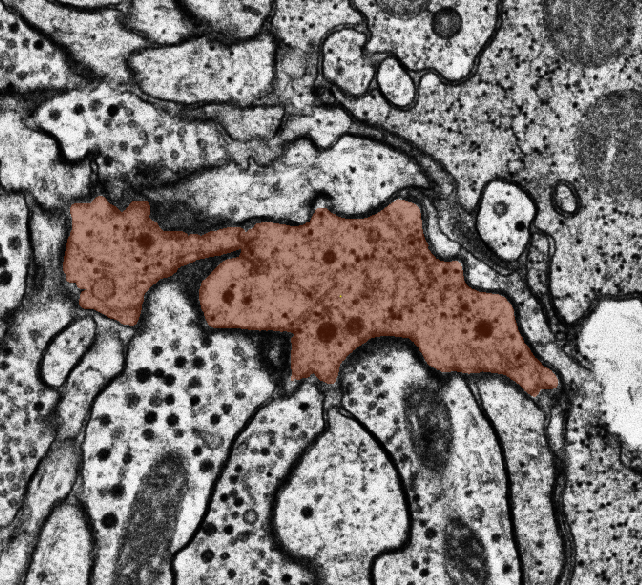
\includegraphics[width=4.9cm]{em1.png}};
  \draw[teald, line width=0.7pt, rounded corners=2pt] (em.south west) rectangle (em.north east);
  \node[font=\scriptsize\itshape, text=teald] at (0,-1.35){one thin neurite (salmon) among crowded neighbours};
  \node[bul, text width=6.2cm] at (0,-3.05)
    {\textbullet\ thin neurites, a few px wide at scale-8\\[2pt]
     \textbullet\ densely packed, many touching\\[2pt]
     \textbullet\ branch / merge points break tracking\\[2pt]
     \textbullet\ $\sim$300 neurons, thousands of chains\\[2pt]
     \textbullet\ single consumer GPU\\[2pt]
     \textbullet\ all-SAM2 (no second dense model yet)};
\end{scope}

% ===== vs =====
\node[circle, draw=spinedraw, fill=white, line width=0.8pt, font=\bfseries, text=spinedraw, inner sep=2pt] at (0,0.4) {vs};

% ===== takeaway =====
\node[rounded corners=3pt, fill=spinefill, draw=spinedraw, line width=0.7pt, align=center,
      font=\small, text=inkc, text width=14.0cm, inner sep=7pt] at (0,-5.55)
  {\textbf{Thinner, more crowded, more numerous, and more branched.} Every addition in the pipeline
   diff (chain decomposition, negative prompts, tiered crops, QC, triage, cross-worm evaluation) is a
   response to this regime shift.};
\end{tikzpicture}
\end{document}
